Parameter Object is a design pattern that is used to group logically related method parameters into a separate entity
(usually data class or structure).
The method is then refactored to accept a single parameter object instead of multiple parameters.
The Parameter Object is usually immutable and contains only accessor methods.

Figure~\ref{fig:group_single_entity} demonstrates extraction of 3 parameters \textit{igmpType},
\textit{maxResponseTime} and \textit{groupAddress} into a new class named \textit{IgmpPacket}.
\textit{IgmpPacketWriter} service is then refactored to accept 2 parameters instead of 5 in the method writeIgmpPacket:
\textit{igmpPacket} and \textit{outputStream}.
Class \textit{IgmpPacket} also contains Factory methods for simple creation of different types of IGMP packets.
These Factory methods are responsible for filling in correct constant values for each type of IGMP packet.

\begin{figure}[!htb]
    \centering
    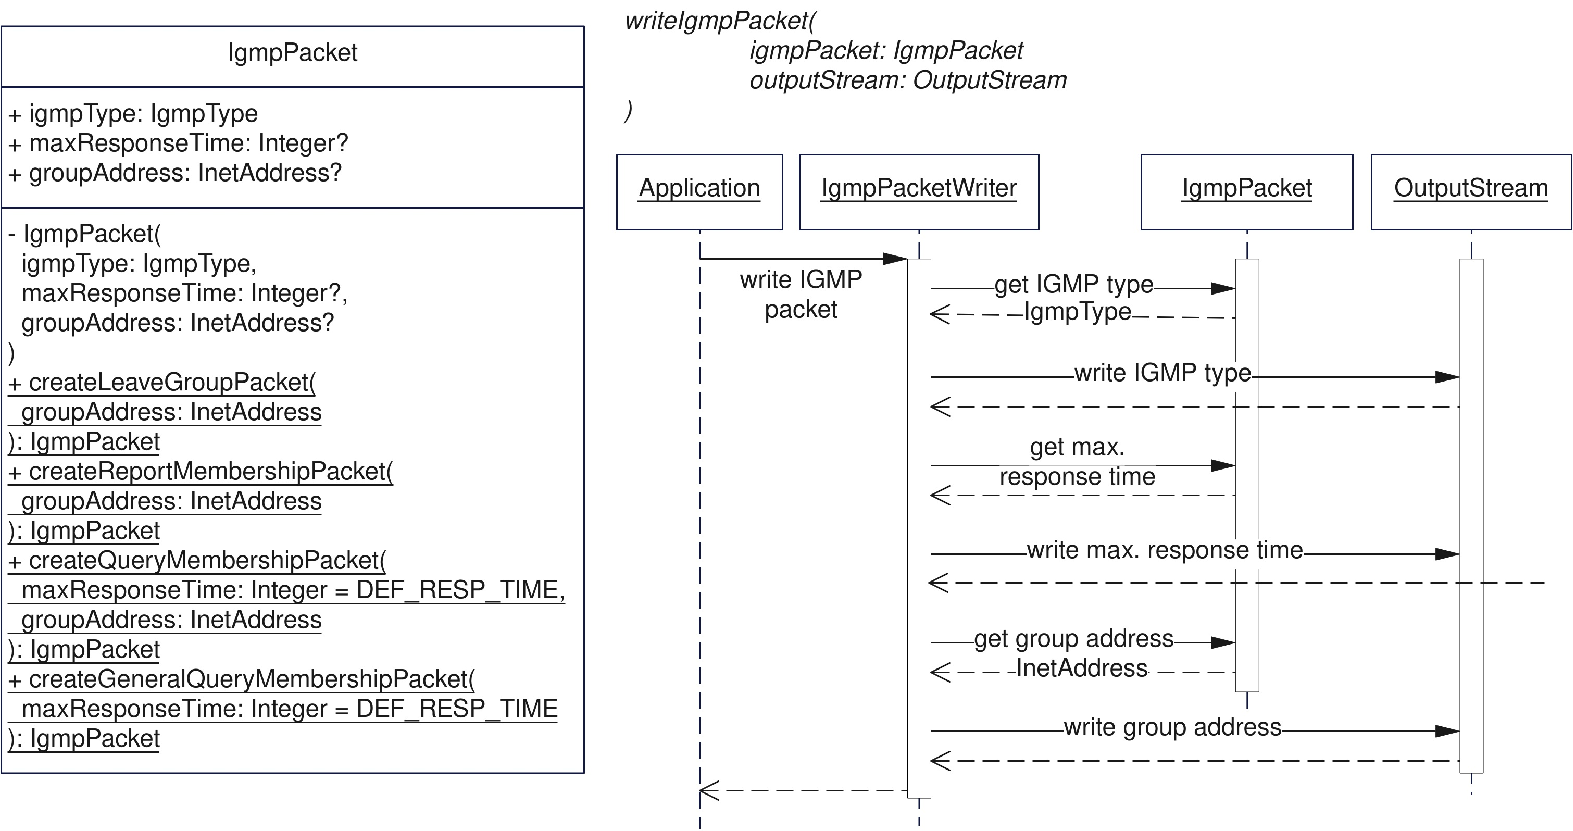
\includegraphics[width=1.0
    \textwidth]{group_single_entity}
    \caption{Parameter Objects: Extraction of a group of parameters into a separate class}
    \label{fig:group_single_entity}
\end{figure}

Instead of using Factory methods, it is possible to use Builder pattern to create
instances of \textit{IgmpPacket} class.
Builder pattern is more suitable if there are many optional parameters that can be set by client.
Figure~\ref{fig:group_build_single_entity} shows how Builder pattern can be used to create an instance
of \textit{IgmpPacket} class.
The whole building process happens in the \textit{build} method that is called by client after setting all necessary
parameters.
Building method usually contains logic around validation of parameters, setting default values, or transformation
of values into a different format.

\begin{figure}[!htb]
    \centering
    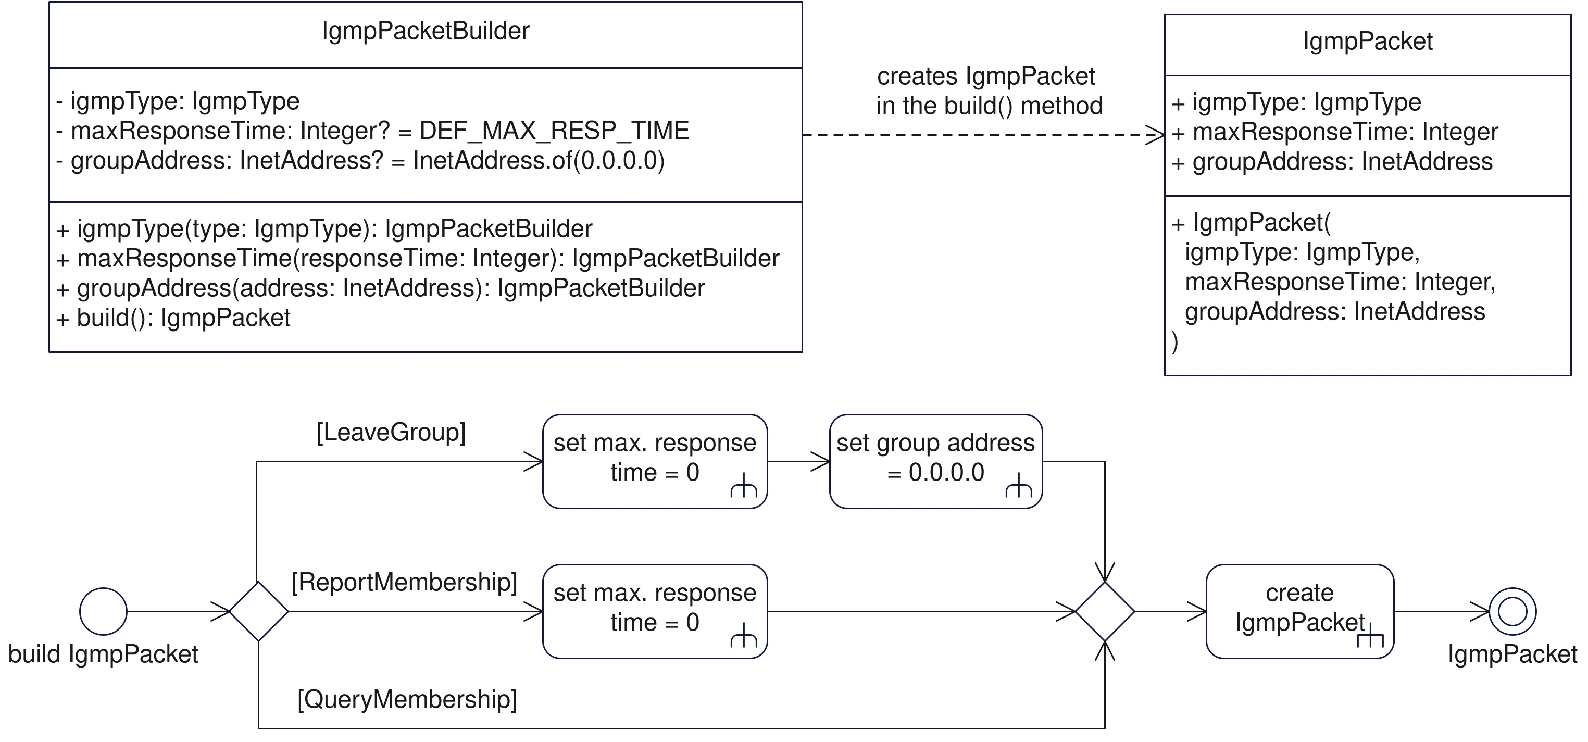
\includegraphics[width=1.0
    \textwidth]{group_build_single_entity}
    \caption{Parameter Objects: Using Builder pattern to create IgmpPacket object}
    \label{fig:group_build_single_entity}
\end{figure}

The following Figures~\ref{fig:group_build_structure} displays next iteration Builder design pattern on this example.
In this case, builder class creates specific instance of \textit{IgmpPacket} subtype - \textit{IgmpLeaveGroupPacket},
\textit{IgmpReportMembershipPacket}, or \textit{IgmpQueryMembershipPacket}.
Definition of multiple subtypes of \textit{IgmpPacket} class is better approach than relying on single entity
if there are multiple structural differences between IGMP packet types or if it is necessary to bound some behavior
to specific type of IGMP packet.
If there is some common behavior or fields that are shared between all IGMP packet types, it is additionally good
to move them to newly created template class that is placed between \textit{IgmpPacket} and its subtypes
in the inheritance structure.

\begin{figure}[!htb]
    \centering
    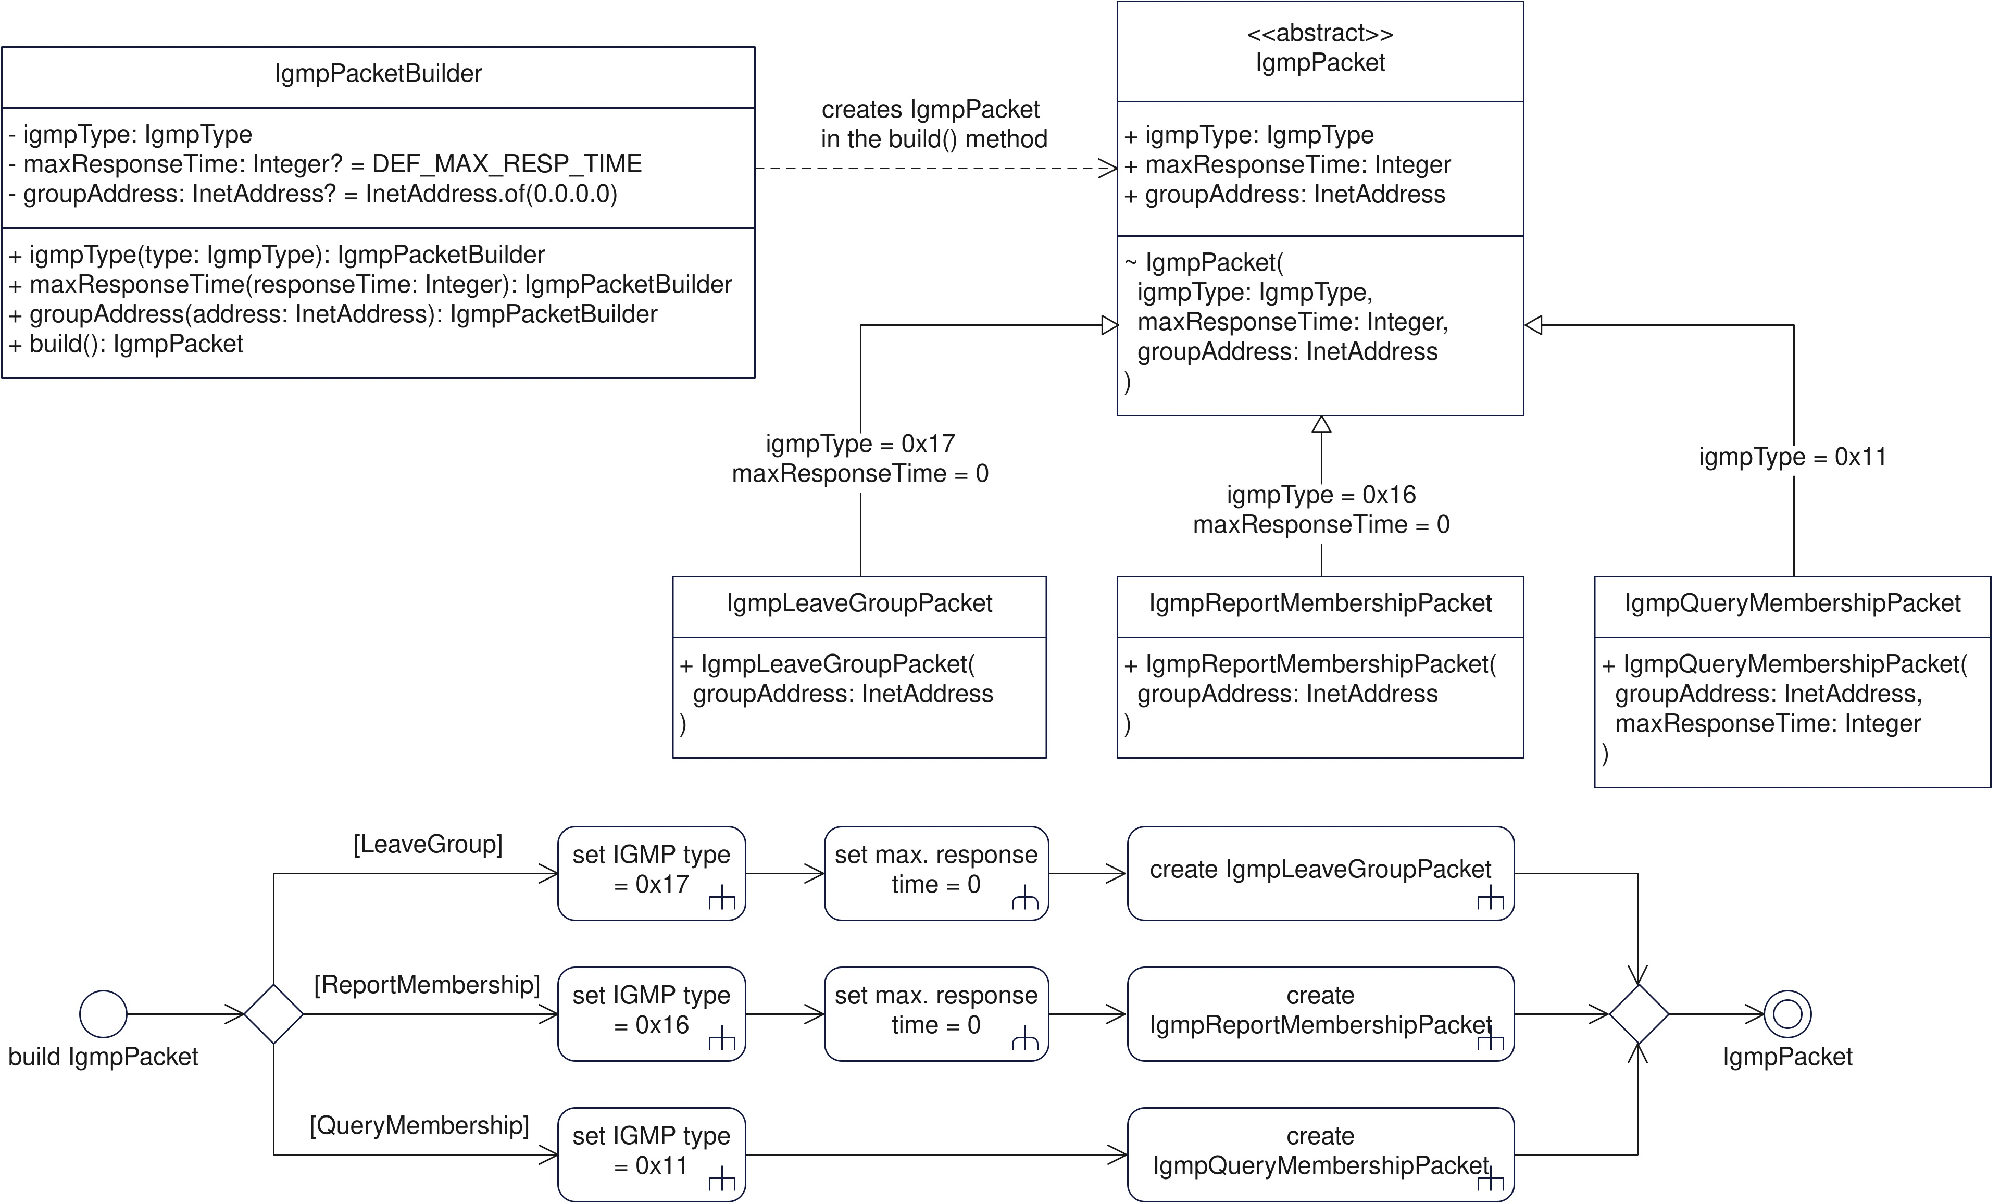
\includegraphics[width=1.0
    \textwidth]{group_build_structure}
    \caption{Parameter Object: Using Builder pattern to create object of IgmpPacket subtype}
    \label{fig:group_build_structure}
\end{figure}

Sometimes it is better to move responsibility for writing IGMP packet to output stream from \textit{IgmpPacketWriter}
to \textit{IgmpPacket} itself.
This is demonstrated in the Figure~\ref{fig:group_write_from_igmp_packet}.
The advantages of this approach is that it is possible to use polymorphism to invoke correct method for writing
IGMP packet to output stream and \textit{IgmpPacketWriter} does not have to access exposed fields
of \textit{IgmpPacket} class.
The disadvantage is that \textit{IgmpPacket} is now tightly coupled with \textit{OutputStream} and maybe
other serialization business logic.
Since \textit{IgmpPacket} is part of the public API such coupling between implementation and API can be problematic
in the future from the view of dependency management and code maintainability.

\begin{figure}[!htb]
    \centering
    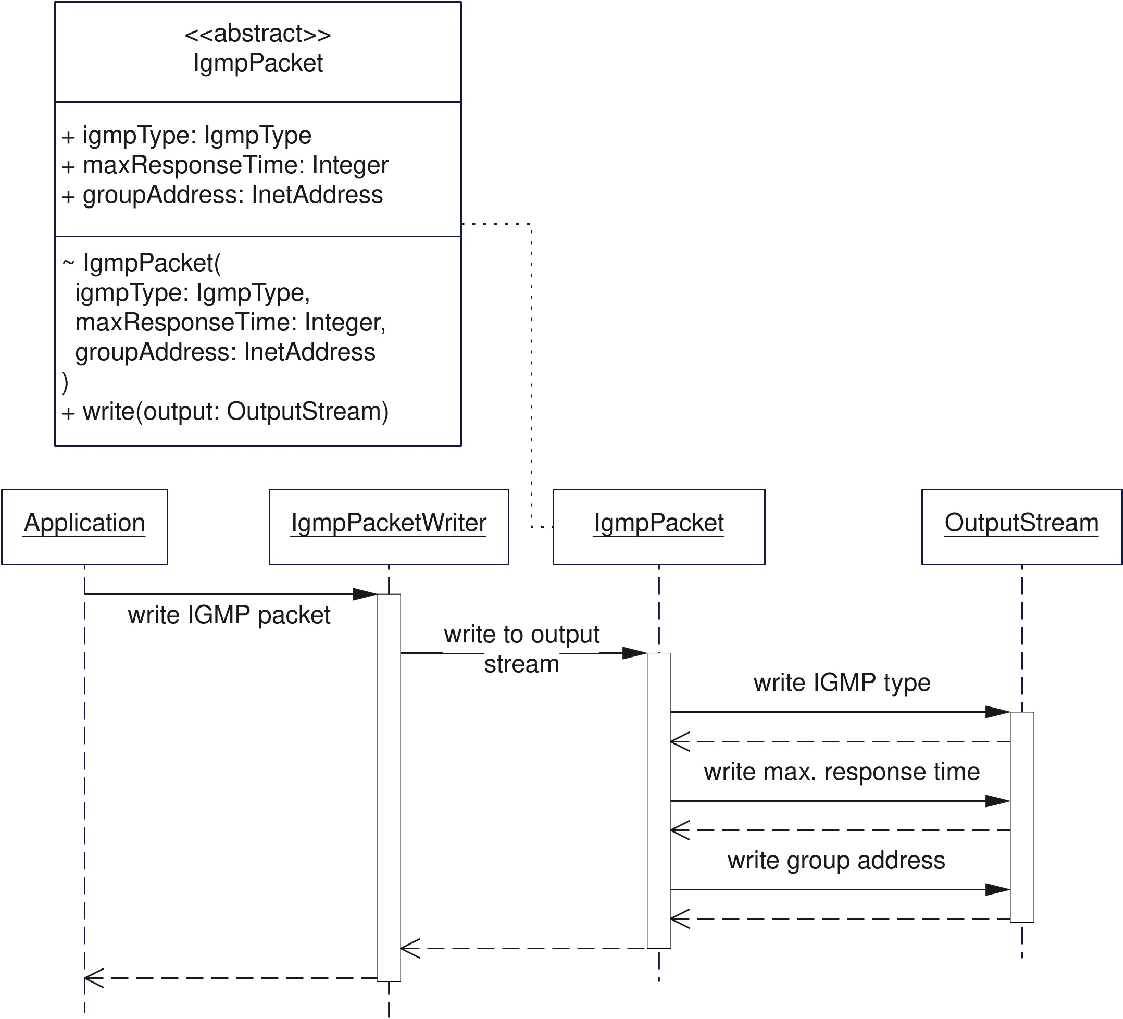
\includegraphics[width=0.8
    \textwidth]{group_write_from_igmp_packet}
    \caption{Parameter Object: Moving write responsibility from IgmpPacketWriter to IgmpPacket}
    \label{fig:group_write_from_igmp_packet}
\end{figure}

The last variation of Parameter Object approach is shown in the Figure~\ref{fig:group_visitor} with
applied Visitor design pattern.
In this scenario, \textit{IgmpPacket} class accepts \textit{IgmpPacketProcessor} as a parameter
in the method \textit{process}.
\textit{IgmpPacketProcessor} represents the interface and \textit{IgmpPacketWriter} implements this interface
- there is one method implementation for each subtype of \textit{IgmpPacket}.
The advantage of this approach in comparison with previous on Figure~\ref{fig:group_write_from_igmp_packet}
is that \textit{IgmpPacket} is not directly coupled with implementation logic.
Rather, there is another abstraction layer between \textit{IgmpPacket} and \textit{IgmpPacketWriter} in form
of generic visitor interface \textit{IgmpPacketProcessor}.
Disadvantage of this approach is the presence of double-dispatching mechanism and the additional implementation
complexity connected with it.

\begin{figure}[!htb]
    \centering
    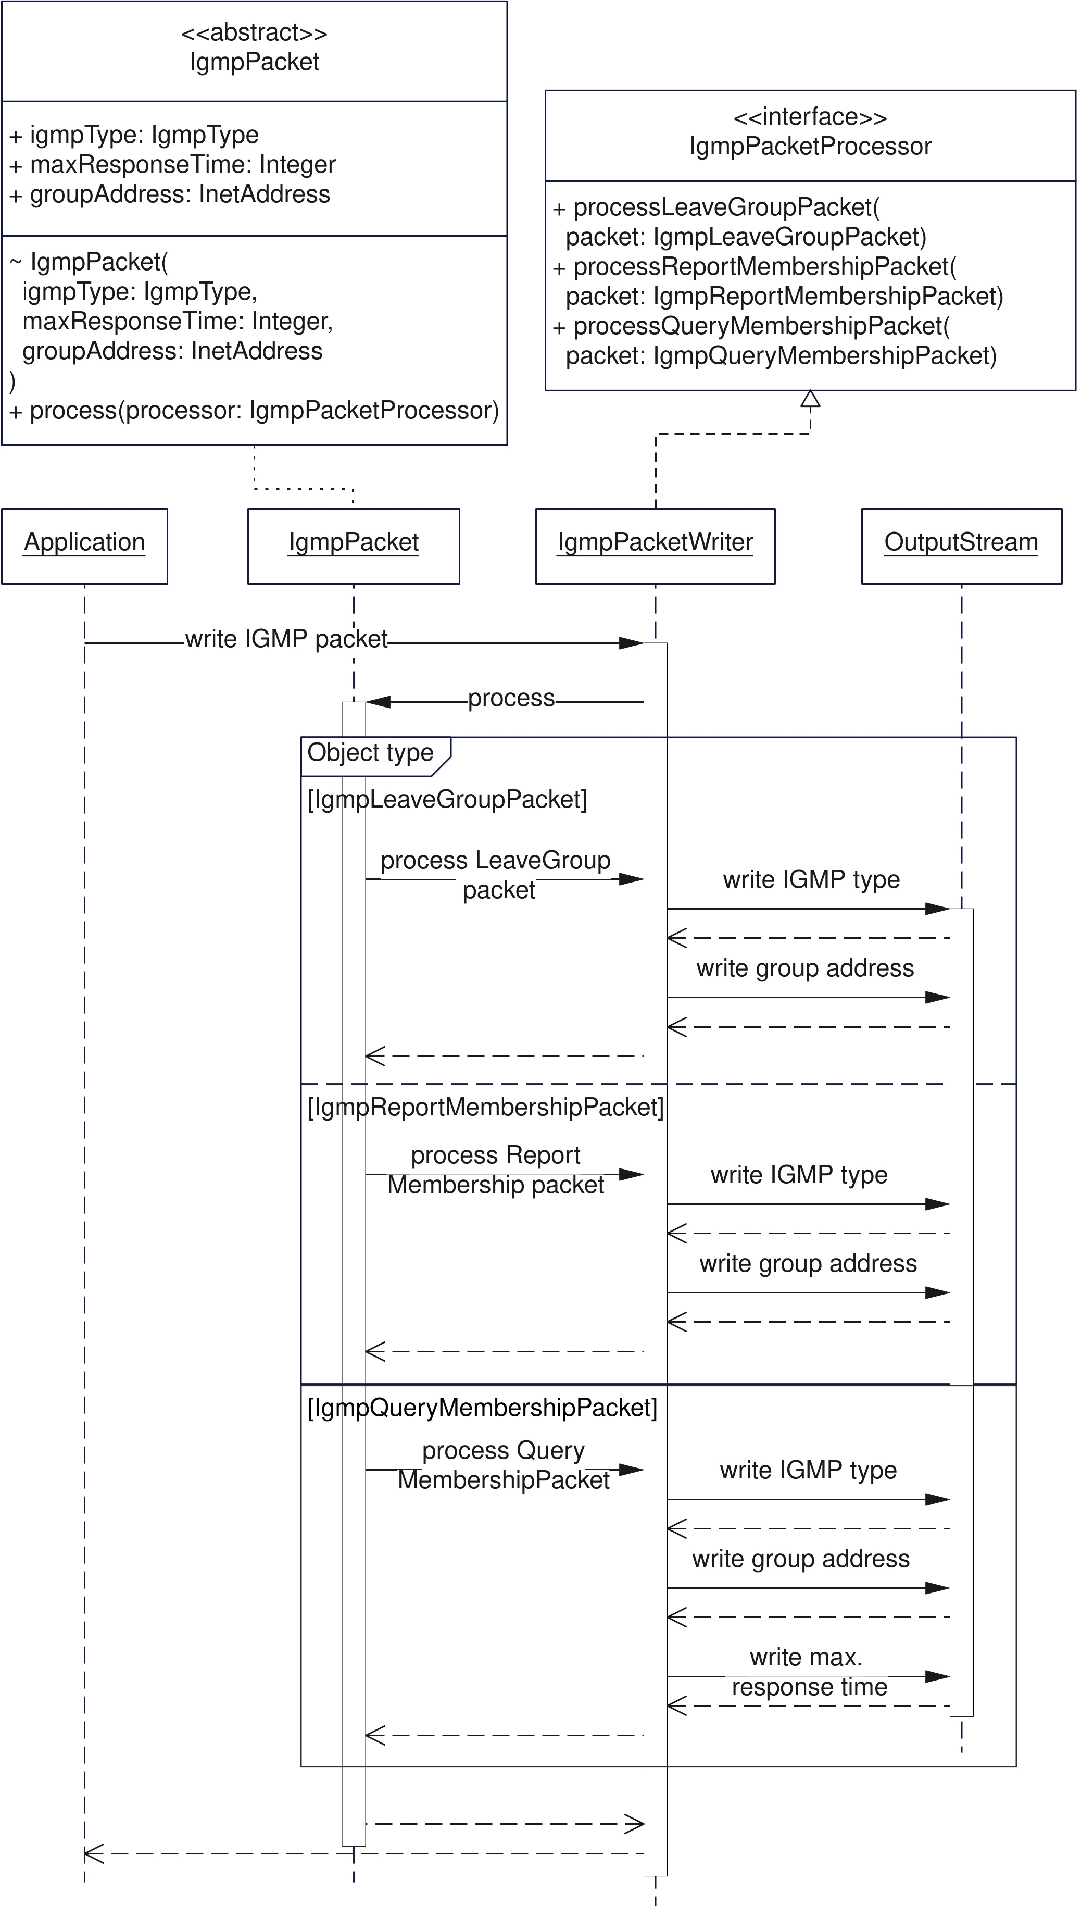
\includegraphics[width=0.75
    \textwidth]{group_visitor}
    \caption{Parameter Objects: Using Visitor design pattern to invoke actions on IgmpPacket subtype}
    \label{fig:group_visitor}
\end{figure}

Benefits of the Parameter Object design pattern:

\begin{itemize}
    \item Grouping of closely related parameters into a single entity improves readability of the code.
    It is also possible to create multiple Parameter Objects that are used in the same method.
    \item Parameter Object can be reused in multiple interface methods and also in the implementation of these methods.
    \item It makes API less fragile, if construction of Parameter Object is done by Builder or Factory pattern
    and not directly by calling constructor of the created class.
\end{itemize}

Drawbacks of the Parameter Object design pattern:

\begin{itemize}
    \item Risk of encapsulation violation if Parameter Object is mutable.
    \item Parameter Object can be overused, and it can lead to creation of too many classes.
    \item Higher risk of exposing implementation details though API that uses this design pattern.
\end{itemize}

Common use-cases of the Parameter Object design pattern:

\begin{itemize}
    \item Compressing long list of parameters into single or just few Parameter Objects.
    \item Grouping optional parameters into Parameter Object and this way avoid method overloading
    and existence of nullable parameters.
    \item Assuring consistency of method definitions by grouping the repetitive list of parameters
    into Parameter Object.
\end{itemize}
